%%%%%%%%%%%%%%%%%%%%%%%%%%%%%%%%%%%%%%%%%%%%%%%%%%%%%%%%%%%%%%%%%%
%%%%%%%%			PRIOR ART
%%%%%%%%%%%%%%%%%%%%%%%%%%%%%%%%%%%%%%%%%%%%%%%%%%%%%%%%%%%%%%%%%%

\subsection{Prior Art}

\paragraph{}
For a thorough research project to be completed, devices that have already been designed, tested and created must be research and analysed. With the popularity of DC power systems increasing in recent years, there have been an many more academics assessing the possibilities. Due to the predominately theoretical design nature of this report and similar aspects of previous papers, a significant focus was made on previous papers.  

\subsubsection{Previous Thesis: Extra-Low Voltage In-Home Power Distribution and Storage}

\paragraph{}
Steven Donohue completed his undergraduate thesis under Geoffery Walker in 2014 \cite{Donohue2014}. This paper assessed various aspects of the similar topic question but specifically focussed on using low voltage DC electricity in homes to power lighting systems. He also considered battery storage solutions and discovered that 48 V DC was the best option for voltage levels for this application \cite{Donohue2014}. He proposed that an installation model for low voltage distribution was uneconomical with current solar feed-in tariffs \cite{Donohue2014}. The final discussion of lighting application proved to be successful using LED lighting circuits in home. Donohue's project will be an asset to the completion of this thesis as the overall concept is very similar. It will be possible to make some assumptions and avoid investing time on smaller calculations due to Donohue's extensive research.         

\subsubsection{Previous Thesis: DC Supply In Buildings}

\paragraph{}
From the University of Science and Technology in Norway, Aurora Bøhle Foss completed her master's thesis on incorporating DC supply into buildings with a larger focus on commercial buildings \cite{Foss2014}. Her focus wasn't specifically on low voltage DC however it did incorporate some research and testing into the feasibility of these systems. Her research found that the most important aspect of incorporating DC supplies into power systems is a highly efficient Voltage Source Converter (VSC). She determined that if a load is requiring AC, it is more efficient to use an AC source. It has been found that higher power loads and cable lengths longer than 10 metres using  1.5 \si{mm^2} and  2.5 \si{mm^2} are impossible due to severe losses.



\subsubsection{Concept: Remote Area Power Supplies}

\paragraph{}
Remote are power supplies (RAPS) are utilised in situations where access to main power grid is either non-existent or untrustworthy \cite{Mendis2010}. They can be created in a variety of ways with gas and diesel generators being popular but expensive \cite{Mendis2010}. Specific to this project, recently renewable energy generation methods have been used to install power systems in these areas. By designing a successfully performing solar panel, battery and converter these locations can have acccess to much needed electricity \cite{Zahedi}. Ahmad Zahedi from Monash University, Australia has designed a solar battery power supply for the purpose of helping nursing clinics and vital services in remote communities \cite{Zahedi}. The structure of his system is as follows and is shown in Figure \ref{fig:RAPS_Block}.

\begin{itemize}[noitemsep]
\item PV generators with mechanical support and future plans for sun tracking system
\item Battery storage in series
\item Power conditioning \& control including measurements and monitoring
\item Buck-Boost regulator
\end{itemize}  

\begin{figure}[H]
\hfill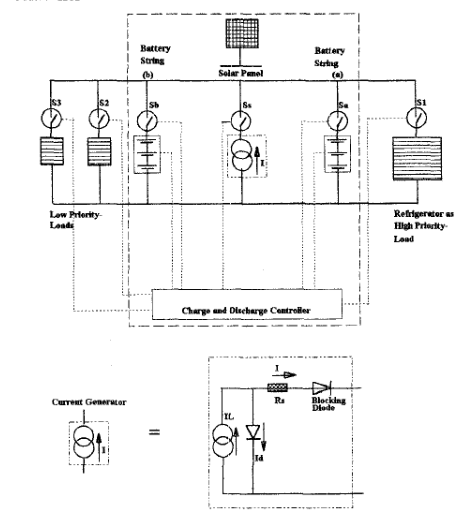
\includegraphics[width = 140mm, height = 110mm]{images/RAPS_Block}\hspace*{\fill}
\caption{{Block Diagram for Photovoltaic RAPS System \cite{Zahedi}}}
\label{fig:RAPS_Block}
\end{figure}        


\subsubsection{Concept: DC Data Centre}

\paragraph{}
Interest in 400 V DC power systems has also been increasing in recent years for applications in telecommunications and data centres \cite{Lisy2015}. Sara Lisy and Mirna Smrekar from Emerson Network Power produced a paper with three case studies of DC powered telecommunication buildings with one case being how an existing -48 V DC large telecom site is powered by 400V DC distribution \cite{Lisy2015}. This application has 400 V DC cabinates that distribute power over long cables to 400 V DC to 48 V DC converters located near the -48 V DC load \cite{Lisy2015}. This was done to minimise the amount of copper used by converter an entire 48 V DC system to a 400 V DC and 48 V DC combination.

\paragraph{}
The site supports an 80 kW load. Initially, two 120 kW 400 V DC power systems ill be installed to support a maximum of 2000 A of -48 V DC end loads. Each system is built up of eight, 15 kW modular rectifiers and expansion is made possible in future. Each side has four, 336 V DC battery strings comprising of 28 12 V DC cells connected to the power system for up to 4 hours of backup in the event of AC failure. This is shown in Figure \ref{fig:DC_Centre}. 

\begin{figure}[H]
\hfill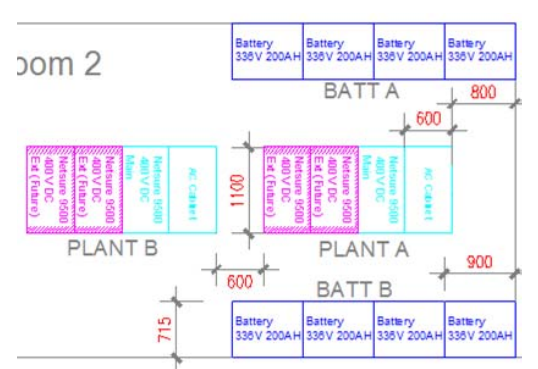
\includegraphics[width = 100mm, height = 80mm]{images/DC_Centre}\hspace*{\fill}
\caption{{Floorplan of DC Backup Data Centre \cite{Lisy2015}}}
\label{fig:DC_Centre}
\end{figure} 

\subsubsection{Concept: Low Voltage Substations DC for Mining Sites}

\paragraph{}
Low Voltage DC distribution is used in some mining sites including underground mines \cite{Morley1990}. This is used for a variety of purchases but predominately at 550\,V\,DC or 250\,V\,DC for machinery \cite{Morley1990}. These machines are locomotives and face equipment and generally a polyphase rectifier circuit is employed for the AC mains \cite{Morley1990}.

\paragraph{}
A related design system launched in 2015 is the ABB's prefabricated DC rail system \cite{website:ProQuest1}. These are modular substations designed to save time and money when working in both the real estate and mining sector within Australia \cite{website:ProQuest1}. These modular power systems offer flexible, adaptable and portable solutions to supplying DC power to devices. Each unit comes with preassembled with 11, 22 or 44 kV switchgear with a rectifier for 750\,V\,DC to 1500\,V\,DC \cite{website:ProQuest1}. Theyare self-contained and indlcue an integrated power supple which reduces risk of power loss overall \cite{website:ProQuest1}.            

\subsubsection{Product: Emphase Micro-Inverters}

\paragraph{}
A competitor to the system that will be designed throughout this thesis will be recent developments in micro-inverter technologies by Enphase \cite{website:Enphase}. These products are designed to be efficient, small and affordable to allow for the DC electricity generated by photo-voltaic cells to be converted to 240V 50Hz AC for the mains. A wide range of fittings are possible depending on the PV cells and switchboard distribution. They have a rated efficiency of 95.7\% \cite{website:Enphase}. 

\subsubsection{Product: Existing Extra Low Voltage DC in Commercial LED Ballasts}

\paragraph{}
TO BE COMPLETED
 
\newpage